\subsection{Dataset: Recorridos 2018}
\begin{enumerate}
    \item \underline{Bici_id_usuario:} dato numérico entero utilizado para identificar al usuario quien realiza el viaje. El mismo es asignado al momento de registrarse al sistema. De los viajes realizados en 2018 se desprende que 121.015 usuarios distintos usaron el sistema. No hay datos faltantes en este campo.
    \item \underline{Bici_Fecha_hora_retiro:} dato categórico ordenado que representa la fecha y la hora del retiro de la bicicleta de la estación en formato aaaa-mm-dd hh:mm:ss. Analizando los valores del atributo encontramos que todas las fechas tienen como año el 2018. No hay datos faltantes en este campo.
    \item \underline{Bici_tiempo_uso:} dato categórico ordenado que representa el tiempo de uso/viaje del viaje en cuestión. Su formato es cantidad "days" hh:mm:ss.
        \begin{itemize}
            \item \textbf{Porcentaje de dato faltante:} 1,67 \%
        \end{itemize}    
    \item \underline{Bici_nombre_estacion_origen:} dato categórico correspondiente al nombre de la estación de bicicletas en la cual se retiro la misma para realizar el viaje. El atributo no tiene datos faltantes.
        \begin{itemize}
            \item \textbf{Cantidad de valores distintos:} 199
            \item \textbf{Moda:} Facultad de Medicina
            \item \textbf{Frecuencia:}
\begin{figure}[H]
    \centering
    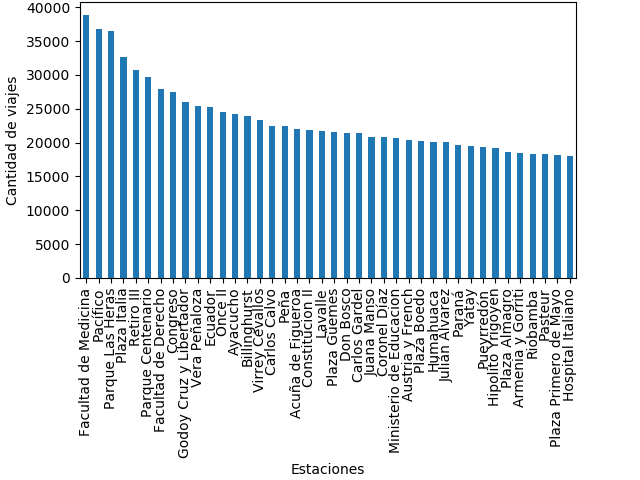
\includegraphics[scale=0.8]{imagenes/nombreOrigenEst1.png}
    \caption{Primeras 40 estaciones.}
 \label{fig: cluster}
\end{figure}

\begin{figure}[H]
    \centering
    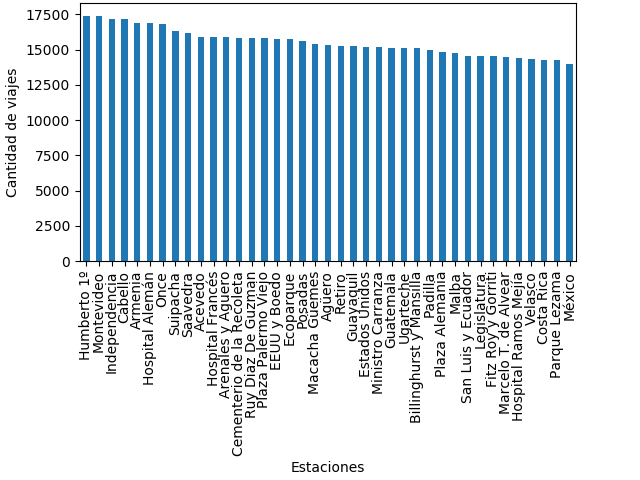
\includegraphics[scale=0.8]{imagenes/nombreOrigenEst2.png}
    \caption{Segundas 40 estaciones.}
 \label{fig: cluster}
\end{figure}

\begin{figure}[H]
    \centering
    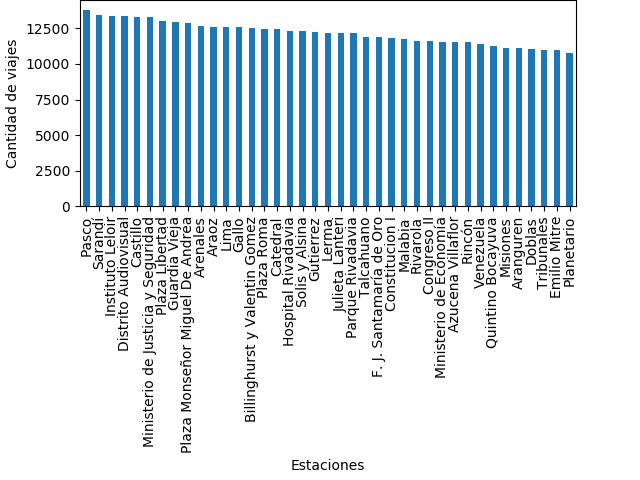
\includegraphics[scale=0.8]{imagenes/nombreOrigenEst3.png}
    \caption{Terceras 40 estaciones.}
 \label{fig: cluster}
\end{figure}

\begin{figure}[H]
    \centering
    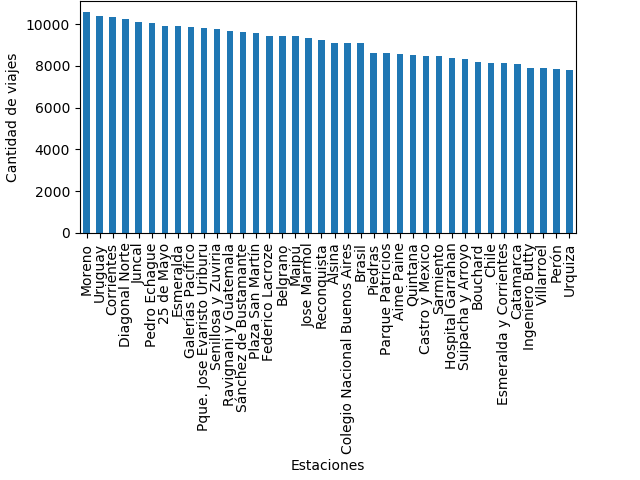
\includegraphics[scale=0.8]{imagenes/nombreOrigenEst4.png}
    \caption{Cuartas 39 estaciones.}
 \label{fig: cluster}
\end{figure}

\begin{figure}[H]
    \centering
    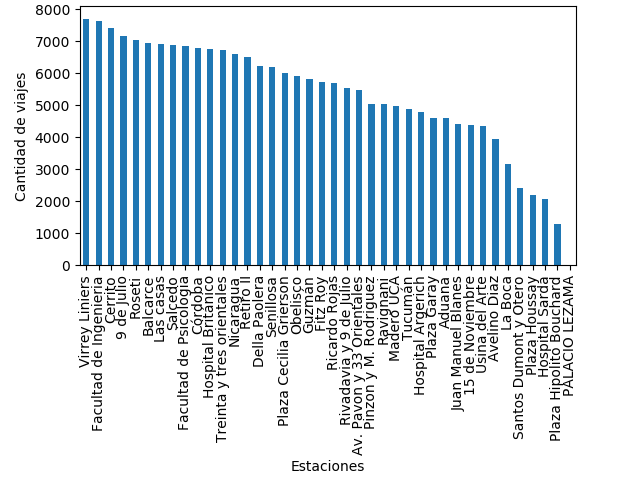
\includegraphics[scale=0.8]{imagenes/nombreOrigenEst5.png}
    \caption{Ultimas 40 estaciones.}
 \label{fig: cluster}
\end{figure}
El outlier PALACIO LEZAMA con tan solo 5 viajes podría ser potencialmente un dato erróneo, teniendo en cuenta el rango de valores que manejan el resto de las estaciones.
        \end{itemize}    
    \item \underline{Bici_estacion_origen:} dato numérico entero que representa el id del Atributo Nombre Estacion Origen. El atributo no tiene datos faltantes.
        \begin{itemize}
            \item \textbf{Cantidad de valores distintos:} 201
            \item \textbf{Moda:} 33
            \item \textbf{Frecuencia:} La frecuencia de este atributo muestra un comportamiento similar al analizado previamente. Sin embargo los últimos 2 ID (505 y 502) con 4 y 1 respectivamente no figuran en el atributo anterior. El análisis bivariado de ambos atributos lo mostramos en la próxima sección.

        \end{itemize}    
    \item \underline{Bici_nombre_estacion_destino:} dato categórico correspondiente al nombre de la estación de bicicletas en la cual se entregó la misma al finalizar el viaje. El atributo no tiene datos faltantes.
        \begin{itemize}
            \item \textbf{Cantidad de valores distintos:} 199
            \item \textbf{Moda:} Facultad de Medicina 
            \item \textbf{Frecuencia:}
 \begin{figure}[H]
    \centering
    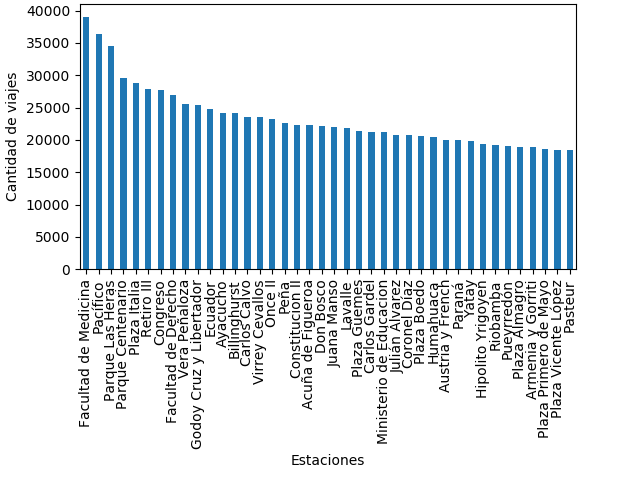
\includegraphics[scale=0.8]{imagenes/nombreDestinoEst1.png}
    \caption{Primeras 40 estaciones.}
 \label{fig: cluster}
\end{figure}

\begin{figure}[H]
    \centering
    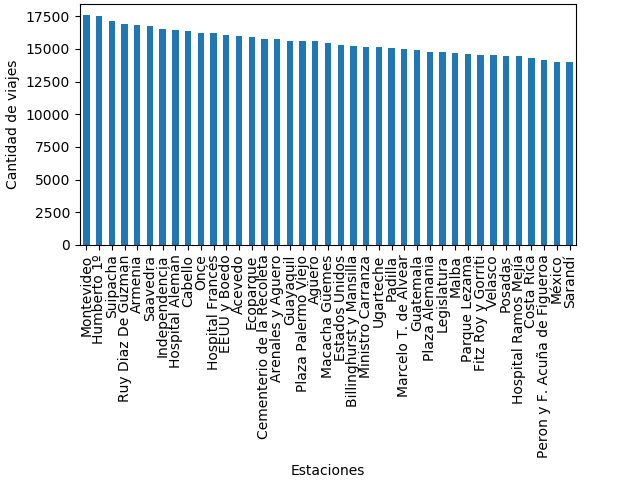
\includegraphics[scale=0.8]{imagenes/nombreDestinoEst2.png}
    \caption{Segundas 40 estaciones.}
 \label{fig: cluster}
\end{figure}

\begin{figure}[H]
    \centering
    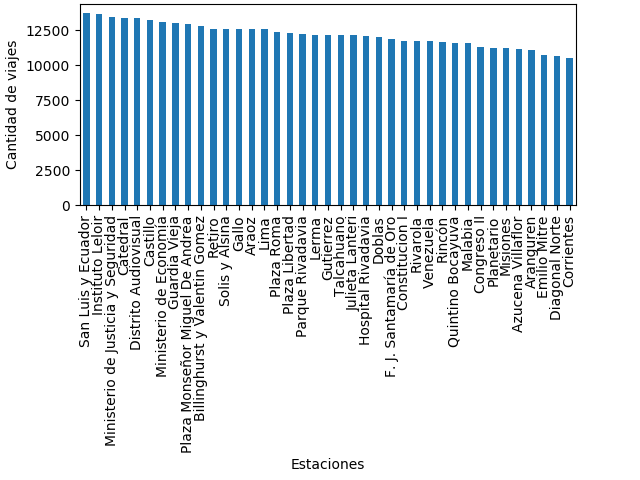
\includegraphics[scale=0.8]{imagenes/nombreDestinoEst3.png}
    \caption{Terceras 40 estaciones.}
 \label{fig: cluster}
\end{figure}

\begin{figure}[H]
    \centering
    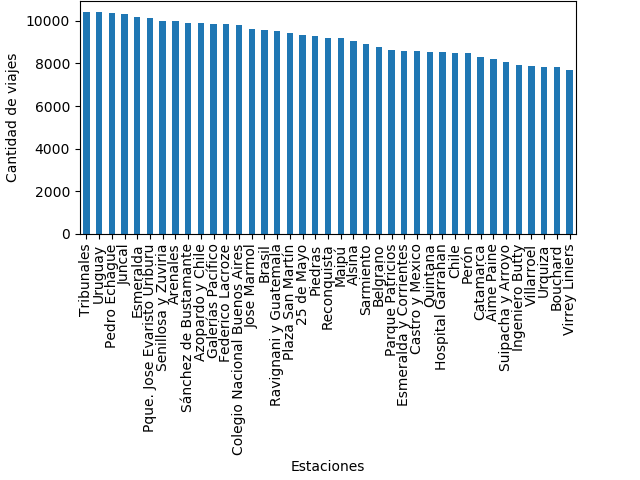
\includegraphics[scale=0.8]{imagenes/nombreDestinoEst4.png}
    \caption{Cuartas 40 estaciones.}
 \label{fig: cluster}
\end{figure}

\begin{figure}[H]
    \centering
    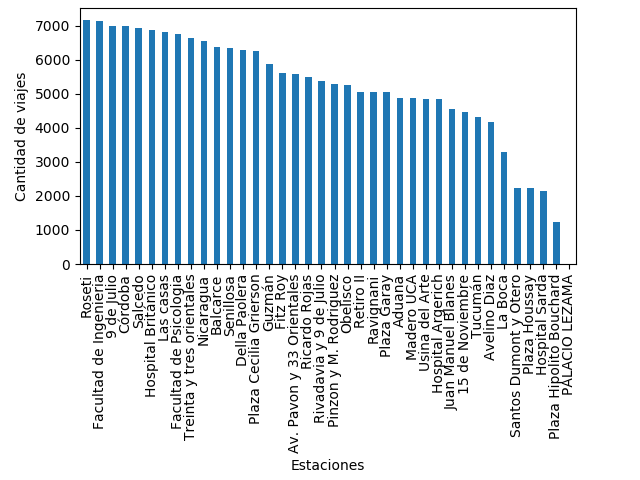
\includegraphics[scale=0.8]{imagenes/nombreDestinoEst5.png}
    \caption{Ultimas 39 estaciones.}
 \label{fig: cluster}
\end{figure}
Nuevamente el outlier PALACIO LEZAMA con tan solo 12 viajes podría ser potencialmente un dato erróneo, teniendo en cuenta el rango de valores que manejan el resto de las estaciones.
        \end{itemize}
    \item \underline{Bici_estacion_destino:} dato numérico entero que representa el id del Atributo Nombre Estación Destino. El atributo no tiene datos faltantes.
        \begin{itemize}
            \item \textbf{Cantidad de valores distintos:} 201
            \item \textbf{Moda:} 33
            \item \textbf{Frecuencia:}  Nuevamente la frecuencia de este atributo muestra un comportamiento similar al analizado previamente. Sin embargo hay 2 ID (502 y 505) con 369 y 68 entradas respectivamente que no figuran en el atributo anterior. El análisis bivariado de ambos atributos lo mostramos en la próxima sección.
        \end{itemize}
    \item \underline{Bici_sexo:} dato categórico nominal que puede tener uno de los siguientes valores: M, F o N. Corresponde al sexo biológico de la persona. Suponiendo que el valor N corresponde a un dato faltante, las métricas son las siguientes:
       \begin{itemize}
            \item \textbf{Porcentaje de dato faltante:} 0,003 \%
            \item \textbf{Frecuencia:} 71,78 \% M y 28,21 \% F
            Observamos una gran desproporción entre hombres y mujeres en el uso del sistema. Sin embargo no tenemos indicios que esto se deba a la calidad del atributo.
        \end{itemize}    
    \item \underline{Bici_edad:} dato numérico entero que corresponde a la edad de la persona.
        \begin{itemize}
            \item \textbf{Valores Min-Max:} 16-140
            \item \textbf{Mediana:} 30
            \item \textbf{Moda:} 28
            \item \textbf{Distribución de los datos:}
\begin{figure}[H]
    \centering
    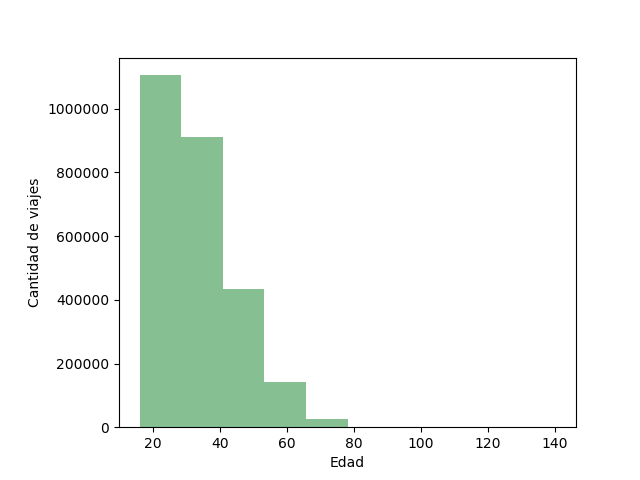
\includegraphics[scale=0.8]{imagenes/edad.png}
    \caption{Cantidad de viajes por edad}
 \label{fig: cluster}
\end{figure}
Si hacemos un zoom en los viajes realizados por personas mayores a 80 años tenemos los siguientes datos:
\begin{figure}[H]
    \centering
    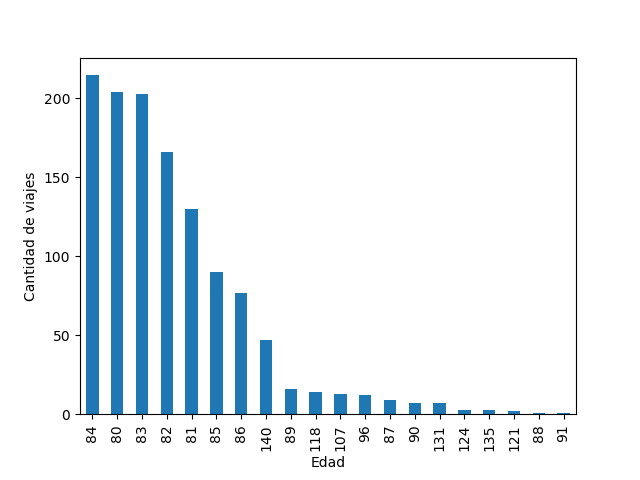
\includegraphics[scale=0.8]{imagenes/edadMayores.png}
    \caption{Cantidad de viajes por personas mayores a 80}
 \label{fig: cluster}
\end{figure}
Claramente nos encontramos con valores anómalos, tenemos edades que son datos erróneos, tales como: 140, 118, 107, 131, 124, 135 y 121.
        \end{itemize}    
\end{enumerate}

\subsection{Dataset: Usuarios 2018}
\begin{enumerate}
    \item \underline{Usuario_id:} dato numérico entero utilizado para identificar al usuario. El atributo no tiene datos faltantes.
    \item \underline{Usuario_sexo:} dato categórico nominal que puede tener uno de los siguientes valores: M, F o O. Corresponde al sexo biológico de la persona. El unico caso faltante/erroneo corresponde al valor 0. Mas allá de este detalle, el atributo no tiene datos faltantes.
       \begin{itemize}
            \item \textbf{Cantidad de datos faltantes/erroneos:} 1
            \item \textbf{Frecuencia:} 54,47 \% M y 45,53 \% F
        \end{itemize}
    No observamos una distribución inusual
    \item \underline{Usuario_edad:} dato numérico entero que corresponde a la edad de la persona.
        \begin{itemize}
            \item \textbf{Valores Min-Max:} 0-160
            \item \textbf{Media:} 32,9
            \item \textbf{Mediana:} 30
            \item \textbf{Moda:} 26
            \item \textbf{Distribución de los datos:}
\begin{figure}[H]
    \centering
    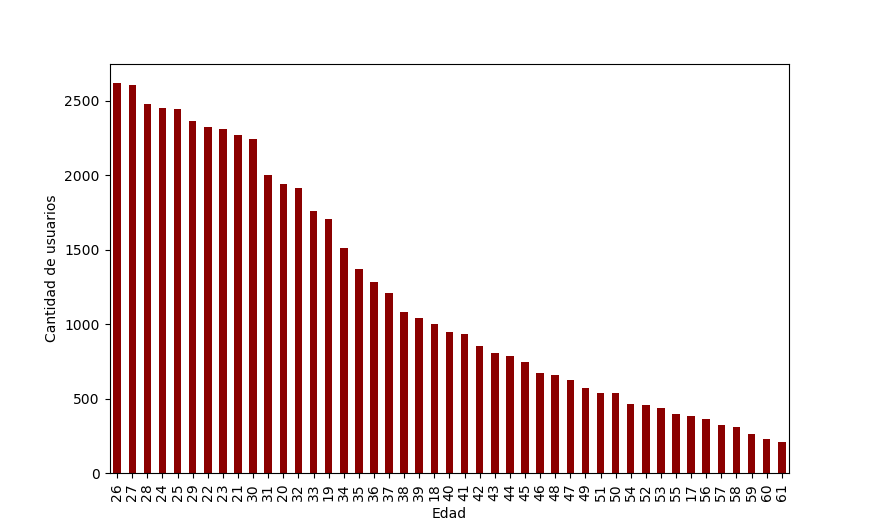
\includegraphics[scale=0.7]{imagenes/edadU1.png}
    \caption{Cantidad de usuarios por edad. Gráfico 1/2}
 \label{fig: cluster}
\end{figure}
\begin{figure}[H]
    \centering
    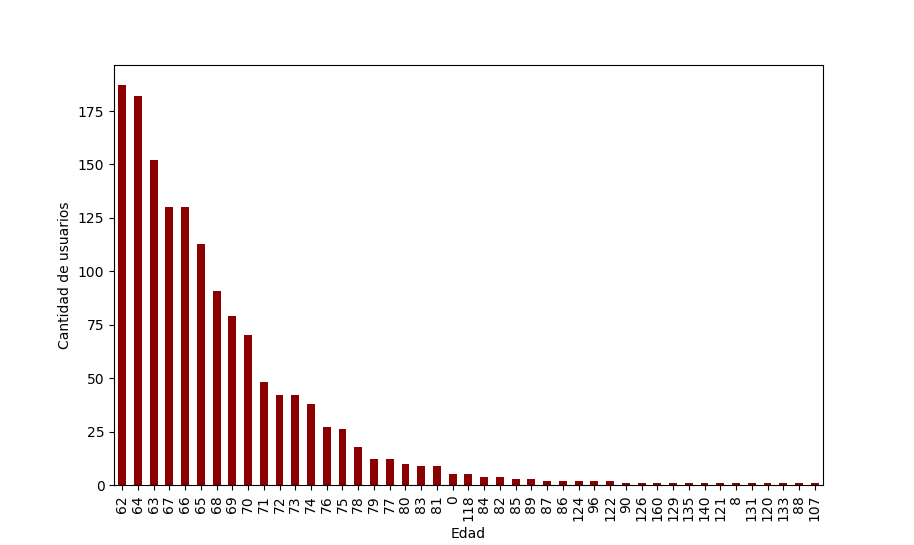
\includegraphics[scale=0.7]{imagenes/edadU2.png}
    \caption{Cantidad de usuarios por edad. Gráfico 2/2}
 \label{fig: cluster}
\end{figure}
 El análisis de la distribución de los datos muestra la existencia de datos erróneos tales como los casos de edad 0, 118, 124, 122, 126, 160, 129, 135, 140, 121, 8, 131, 120, 133 y 107. Estos se deben, seguramente, a errores en el proceso de registro de los usuarios.
        \end{itemize}
    \item \underline{Fecha_alta:} dato categórico ordenado que representa la fecha del 
    registro en el sistema en formato dd/mm/aaaa. Este atributo no tiene datos faltantes.
    \item \underline{Hora_alta:} dato categórico ordenado que representa la hora del registro en el sistema en formato h:mm:ss. La particularidad de este atributo es que la hora para todos los nuevos usuarios registrados es las 5, con diversas combinaciones de minutos y segundos. La única explicación que se nos ocurren es que solo en esa hora se cargan al sistema nuevos usuarios. Este atributo no tiene datos faltantes.
\end{enumerate}
